\documentclass[11pt,a4paper]{article}

\usepackage[T1]{fontenc}
\usepackage[utf8]{inputenc}
\usepackage[english]{babel}
\usepackage{lmodern}
%\usepackage{circuitikz}
\usepackage{color}
\usepackage{wrapfig}
\usepackage{placeins}
\usepackage{subfigure}
\usepackage{tabu}
\usepackage{fullpage}
\usepackage[squaren]{SIunits}
\usepackage{graphicx}
%\usepackage[pdftex]{graphicx}
\usepackage{epstopdf}
\usepackage{epsfig}
\usepackage{hyperref}
\usepackage{tikz}
\usepackage{tikz-qtree}
\usepackage{eurosym}
%\usepackage{chemist}
\usepackage{amsmath}
\usepackage{amssymb}
\usepackage{mathrsfs}
\usepackage{dsfont}% use $\mathds{1}$
\newcommand{\C}{\mathbb{C}}
\newcommand{\N}{\mathbb{N}}
\newcommand{\Z}{\mathbb{Z}}
\newcommand{\R}{\mathbb{R}}
\newcommand{\red}{\textcolor{red}}
\newcommand{\dis}{\displaystyle}
\newcommand{\dr}{\partial}
\newcommand{\txt}{\text}
\newcommand{\td}{\todo[inline]}
\newcommand{\ttt}{\texttt}
\newcommand{\itt}{\textit}

\usepackage{algorithm}
\usepackage{todonotes}
\usepackage[noend]{algpseudocode}

%\newtheorem{theoreme}			     {Théorème}	[chapter]
%\newtheorem{proposition}[theoreme]	 {Proposition}	
%\newtheorem{corollaire}	  [theoreme]	 {Corollaire}	
%\newtheorem{lemme}	      [theoreme]  {Lemme}		
%\newtheorem{definition}	         {Définition}[chapter]
%\theoremstyle{definition}
%\newtheorem{exemple}			     {Exemple}	[chapter]
%\newtheorem{contreexemple}[exemple]{Contre-exemple}
%\newtheorem{probleme}	             {Probl\`eme}[chapter]

\usepackage{listings}
\usepackage{textcomp}
\definecolor{listinggray}{gray}{0.9}
\definecolor{lbcolor}{rgb}{0.9,0.9,0.9}
\lstset{
	backgroundcolor=\color{lbcolor},
	tabsize=4,
	rulecolor=,
	language=matlab,
        basicstyle=\scriptsize,
        upquote=true,
        aboveskip={1.5\baselineskip},
        columns=fixed,
        showstringspaces=false,
        extendedchars=true,
        breaklines=true,
        prebreak = \raisebox{0ex}[0ex][0ex]{\ensuremath{\hookleftarrow}},
        frame=single,
        showtabs=false,
        showspaces=false,
        showstringspaces=false,
        identifierstyle=\ttfamily,
        keywordstyle=\color[rgb]{0,0,1},
        commentstyle=\color[rgb]{0.133,0.545,0.133},
        stringstyle=\color[rgb]{0.627,0.126,0.941},
}

\DeclareMathOperator{\e}{e}

\title{Titre}
\author{Florentin Goyens}
\date{\today}

\begin{document}

\tabulinesep=1.2mm
\begin{center}
\hrule
\begin{tabular}{c}
\\[0.005cm]
\Large{Applied Numerical Methods - Computer Lab 2}\\[0.3cm]
\textsc{Goyens} Florentin \& \textsc{Weicker} David \\[0.2cm]
$\text{1}^{\text{st}}$ October 2015\\[0.2cm]
\end{tabular}
\hrule
\end{center}

\section*{Part A. Accuracy of a Runge-Kutta method}
bla bla bla

\section*{Part B. Stability investigation of a Runge-Kutta method}
In this section, we will investigate the stabilty of a Runge-Kutta method. We will study a stiff problem, the Robertson's equations. As a remainder, here is the problem : 

\begin{eqnarray*}
\textbf{x}' =& \left( \begin{array}{c}
-k_1x_1+k_2x_2x_3 \\ 
k_1x_1-k_2x_2x_3-k_3x_2^2 \\ 
k_3x_2^2 
\end{array} \right) \\
\textbf{x} =& \left( \begin{array}{c}
1 \\ 
0 \\ 
0 
\end{array} \right)
\end{eqnarray*}

The problem is stiff because of the practical values of the parameters. In this example, we have $k_1=0.04$, $k_2=10^4$ and $k_3=3 \cdot 10^7$.

\subsection*{B1. Constant stepsize experiment}

We are going to solve the Robertson's problem first with a constant stepsize. The Matlab code can be found at the end of this section. We had to try and see if the method was stable for this problem using different numbers of steps, namely $N = [125, 250, 500, 1000, 2000]$. The answer given by our code was that it was not stable for $N =[125, 250, 500]$. Thus, the smallest number of steps (from the 5 given) needed to obtain a stable solution is $n = 1000$. The solution for the smallest step size ($n = 2000$) is given in figure \ref{robert}.

\begin{figure}
\begin{center}
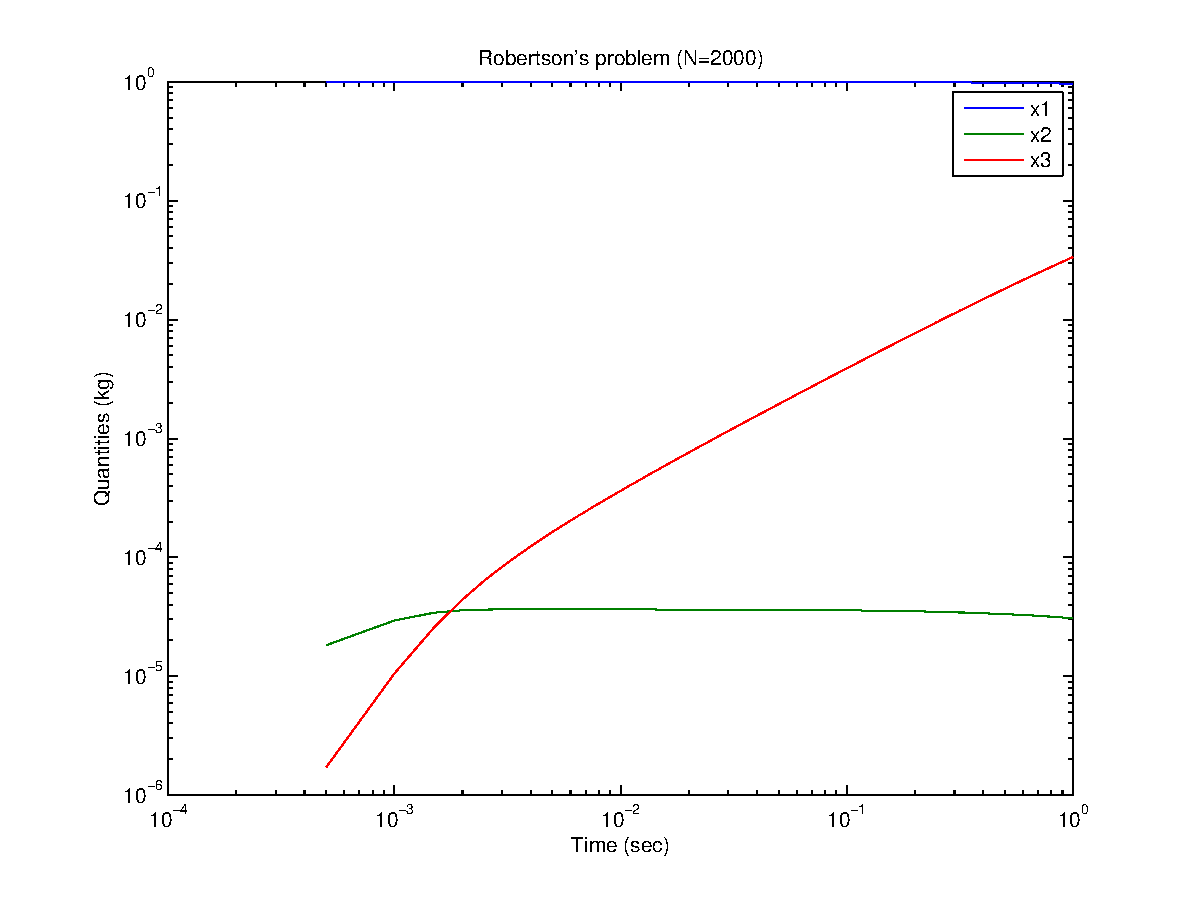
\includegraphics[scale=0.5]{robert.eps}
\caption{Robertson's problem with $n = 2000$}
\label{robert}
\end{center}
\end{figure}
\FloatBarrier

%Ce truc insere mon code MATLAB (nice!) 
\lstinputlisting{LAB2B1.m}

\subsection*{B2. Adaptative stepsize experiment using Matlab functions}

In this section, we are going to use the built-in IVP-solvers. As usual, the code can be found at the end of the section. 

There are many different solvers available. Our first task was to use the non-stiff solver $ode23$ for different relative tolerances (using $odeset$) and for a time span of one second. Then, we were to plot a graph of the step size as a function of time for one of the tolerance. The following table gives the number of steps for each relative tolerance.

\begin{center}
\begin{tabular}{|c|c|}
\hline 
\textbf{RelTol} & \textbf{Number of steps} \\ 
\hline 
$10^{-3}$ & 866 \\ 
\hline 
$10^{-4}$ & 867 \\ 
\hline 
$10^{-5}$ & 868 \\ 
\hline 
$10^{-6}$ & 868 \\ 
\hline 
\end{tabular} 
\end{center}

We can see that the number of step increases but not significantly as the relative tolerance constraint increases. The plot of the stepsize as a function of time for the $RelTol = 10^{-6}$ can be seen in figure \ref{step1}.

\begin{figure}
\begin{center}
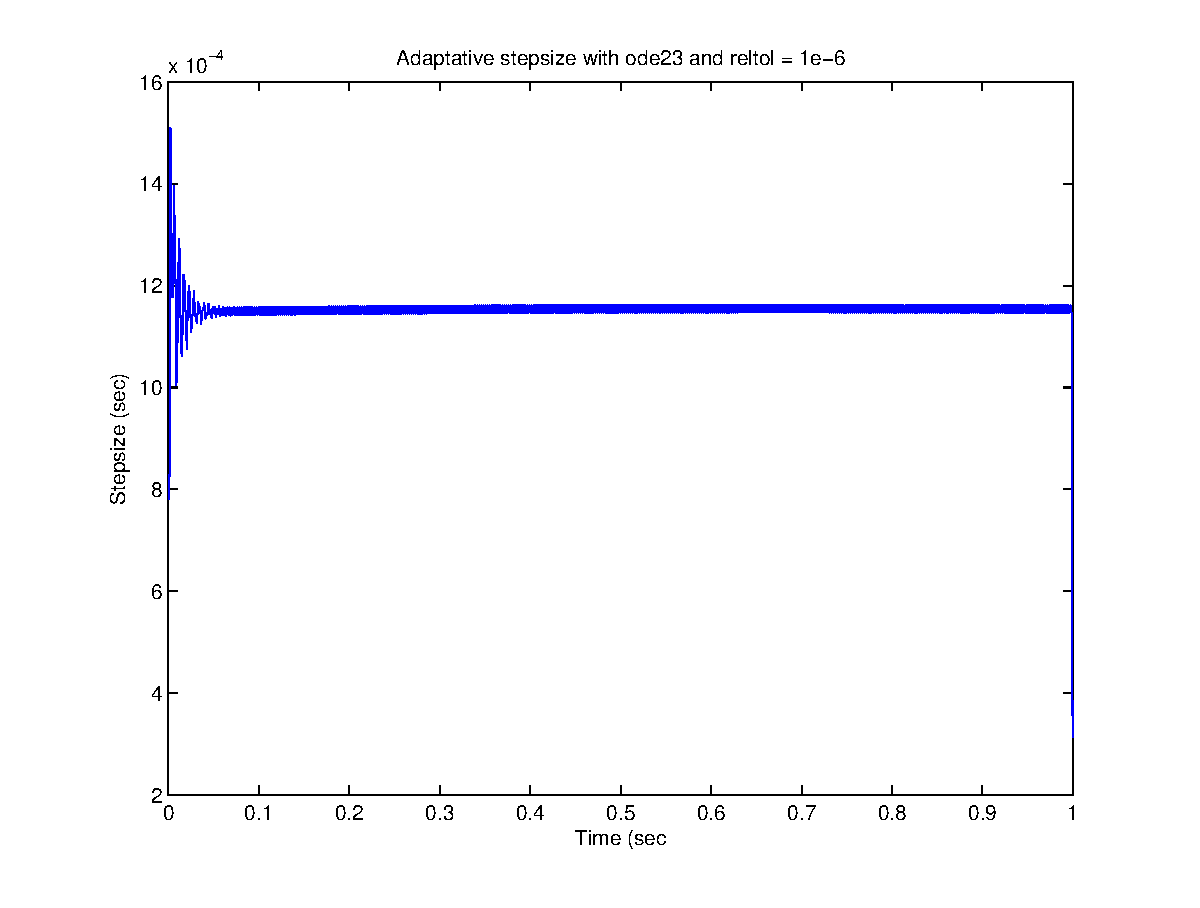
\includegraphics[scale=0.5]{step1.eps}
\caption{Adaptative stepsize with $ode23$ for $RelTol = 10^{-6}$}
\label{step1}
\end{center}
\end{figure}

Even if we can see some oscillations in the beginning, the stepsize appear to stay around the same value. That is hardly adaptative.\\

Our second task was to use a stiff solver, namely $ode23s$, and do the experiment again but for a larger time span, from 0 to 1000 seconds. We obtained the following numbers of step for the given tolerances.

\begin{center}
\begin{tabular}{|c|c|}
\hline 
\textbf{RelTol} & \textbf{Number of steps} \\ 
\hline 
$10^{-3}$ & 30 \\ 
\hline 
$10^{-4}$ & 37 \\ 
\hline 
$10^{-5}$ & 48 \\ 
\hline 
$10^{-6}$ & 62 \\ 
\hline 
\end{tabular} 
\end{center}

First, we can noticed that even though the t-interval is a thousand time longer, the number of steps taken by $ode23s$ is lesser. Second, now the number of steps increases as the relative tolerance constraint increases. That is a good thing because it means that the stepsize is governed by the relative tolerance and not some other factor. We were also asked to plot the stepsize as a function of time for $ode23s$. We choose the same relative tolerance that the one used before, that is $RelTol = 10^{-6}$ This is shown in figure \ref{step2}.

\begin{figure}
\begin{center}
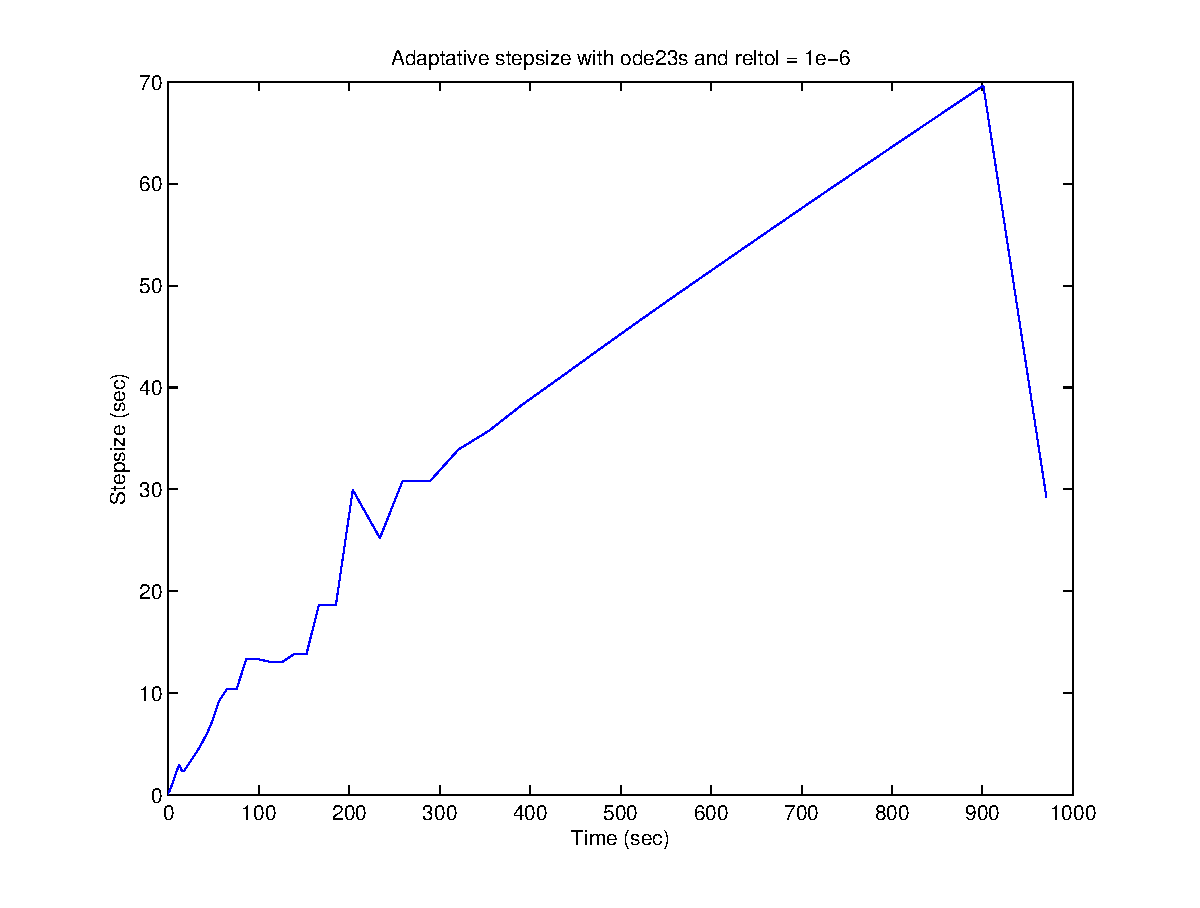
\includegraphics[scale=0.5]{step2.eps}
\caption{Adaptative stepsize with $ode23s$ for $RelTol = 10^{-6}$}
\label{step2}
\end{center}
\end{figure}

We can see that the value of the stepsize is way larger than for $ode23$. This is an example of why a stiff solver is better when confronting a stiff problem.

%Ce truc insere mon code MATLAB (nice!) 
\lstinputlisting{LAB2B2.m}


\section*{Part C. Parameter study of solutions of an ODE-system}
blo blo blo
\end{document}